\documentclass[11pt]{article}
\usepackage[margin=1in]{geometry}
\usepackage{amsmath,amssymb,amsfonts}
\usepackage{graphicx,float}
\usepackage{fancyhdr,booktabs}
\usepackage{listings}
\usepackage{hyperref}
\lstset{
    language=Matlab,
    basicstyle=\ttfamily\small,
    breaklines=true,
    keepspaces=true,
    showstringspaces=false
}

% Header and Footer Setup
\pagestyle{fancy}
\fancyhf{}
\lhead{ME 351 -- Fall 2026}
\rhead{Homework 1}
\cfoot{\thepage}

\title{\textbf{ME 351}\\[0.5ex]\Large Homework 1}
\author{Zeshui Song}
\date{Fall 2026}

\begin{document}
\maketitle

\vspace{-1em}

\subsection*{Exercise 1}
Identify two feedback control systems that interest you and that we have not already discussed in class. Briefly describe the systems and identify:
\begin{itemize}
    \item the sensing mechanism,
    \item the actuation mechanism, and
    \item the computational or decision-making element.
\end{itemize}
Most importantly, for each system, explain what feedback accomplishes. For example, what uncertainty or disturbance does feedback make the system robust to, or what aspect of the system dynamics does feedback modify? Include and properly cite at least one source for each system.

\paragraph{Solution}\mbox{}\\

\noindent\textbf{System 1: Electric Kettle}
\begin{itemize}
    \item Sensing mechanism: A thermistor that measures the temperature of the water inside the kettle.
    \item Actuation mechanism: A switch that turns the heating element on and off.
    \item Computational or decision-making element: The thermistor sends current signals to a controller that turns the heating element on or off based on the temperature reading to maintain the desired water temperature.
    \item Feedback accomplishes: The resulting water temperature is maintained at the desired level despite heat loss to surroundings, turning the heating element back on if the water cools down, and turning it off when it reaches the set temperature.
    \item Source: R. G. Corkin, ``Improved temperature sensor for an electric kettle,''
Australian Patent Application AU 2010224322 A1, Mar. 31, 2011.
[Online]. Available:
\url{https://patents.google.com/patent/AU2010224322A1/en}
\end{itemize}
\textbf{System 2: Refrigerator defrost control}

\begin{itemize}

    \item Sensing mechanism: A thermistor measures the temperature of the evaporator coil.

    \item Actuation mechanism: A defrost heater turns on to melt frost and ice buildup on the evaporator coil.

    \item Computational or decision-making element: The thermistor sends a temperature signal to the refrigerator's electronic control board, which controls the defrost heater.

    \item Feedback accomplishes: During the defrost cycle, the heater melts frost from the evaporator. As the evaporator temperature rises, the thermistor detects the change. Once a cutoff temperature is reached, indicating that the frost has melted, the controller turns the defrost heater off. This prevents excessive frost buildup, which could restrict airflow and reduce refrigerator cooling performance.
    \item Source: D. G. Schenk, J. R. Wisnoski, D. A. Diekmann, and S. J. Kuehl, ``Refrigeration appliance with pulsed defrost heater,'' U.S. Patent 6,694,754 B1, Feb. 24, 2004. [Online]. Available: \url{https://patents.google.com/patent/US6694754B1/en}
\end{itemize}

\subsection*{Exercise 2}
Why do you think feedback control is ubiquitous in biological systems? Answer in a short paragraph.

\paragraph{Solution} This is because biological systems involve very narrow operating ranges for many physiological variables, such as body temperature, blood sugar levels, and blood pressure. Without feedback control, these variables would fluctuate widely due to external disturbances and there would be no mechanism to detect and correct deviations from a healthy state. This would be unideal for the goal of staying alive, which is presumably the most important goal of any biological system.

\subsection*{Exercise 3}
Do Exercise 1.5 from \textit{Feedback Systems: An Introduction for Scientists and Engineers} by \AA str\"om and Murray.\\\\
\textbf{1.5 (Integral action)} We say that a system with a constant input reaches steady state if all system variables approach constant values as time increases. Show that a controller with integral action, such as those given in equations (1.4) and (1.5), gives zero error if the closed loop system reaches steady state. Notice that there is no saturation in the controller.
\begin{equation}
u(t) = k_i \int_0^t e(\tau)\,d\tau
\tag{1.4}
\end{equation}

\begin{equation}
u(t) = k_p e(t)
+ k_i \int_0^t e(\tau)\,d\tau
+ k_d \frac{de(t)}{dt}
\tag{1.5}
\end{equation}

\paragraph{Solution} Looking at the PID controller described by equation (1.5), the integral controller in equation (1.4) can be treated as a special case of the PID controller where the proportional and derivative gains are zero.\\\\
Differentiating equation (1.5) to get rid of the integral gives:
\[
\frac{du(t)}{dt}
=
k_p\frac{de(t)}{dt}
+
k_i e(t)
+
k_d\frac{d^2e(t)}{dt^2}
\]
Since at steady state all system variables approach constant values, the derivative terms go to zero, leaving:
\[
0 = k_i e_{ss},
\qquad
\text{where} \quad e_{ss} = \lim_{t\to\infty} e(t)
\]
Thus, if \(k_i \neq 0\), then
\[
e_{ss}=0,
\]
showing that the steady-state error must be zero.\\\\
Otherwise, a nonzero steady-state error would cause the integral term to continue growing to infinity. Since the controller is assumed to have no saturation (the output is not bounded), the controller output would also continue growing rather than approach a constant value. Therefore, the system would not be at steady state.

\subsection*{Exercise 4}
In this exercise, we investigate how feedback changes the sensitivity of a control system to model uncertainty. Consider a speed-control system with dynamics given by
\[
m\dot{v}=-av+u+d,
\]
where $u$ is the control input (force applied by engine) and $d$ is the disturbance input (force applied by hill, etc.), which will be ignored below ($d=0$). An open-loop feedforward control strategy to achieve a given reference speed $v_{\mathrm{ref}}$ would be to choose
\[
u=\hat{a}v_{\mathrm{ref}},
\]
where $\hat{a}$ is your estimate of $a$, which may not be accurate.

\begin{enumerate}
    \item[(a)] Compute the steady-state response for both the open-loop strategy above and for the proportional (P) feedback law
    \[
    u(t)=-k_p\bigl(v(t)-v_{\mathrm{ref}}\bigr)
    \]
    and compare the steady-state (with $d=0$) as a function of $\beta=a/\hat{a}$ when $k_p=10\hat{a}$.
    \end{enumerate}
\paragraph{Solution} This problem asks how different types of controls affect the steady-state response of a system with model uncertainty (in this case, the uncertainty is in the parameter \(a\)).\\\\
For $d=0$ and at steady state ($\dot{v} = 0$), the equation of motion becomes:
\[0=-av_{ss}+u\]
Plugging in the first open-loop control strategy into the EOM gives:
\[0 = -av_{ss}+\hat{a}v_{\mathrm{ref}}\quad \implies \frac{a}{\hat{a}} = \frac{v_{\mathrm{ref}}}{v_{ss}}\quad \implies \boxed{v_{ss}= \frac{v_{\mathrm{ref}}}{\beta}}\]
Plugging in the proportional feedback control law into the EOM gives:
\[0=-av_{ss}-k_p(v_{ss}-v_{\mathrm{ref}}) \quad \implies \frac{a}{\hat{a}} = 10\left(\frac{v_{\mathrm{ref}}}{v_{ss}}-1\right) \quad \implies \boxed{v_{ss} = v_{\mathrm{ref}}\left(\frac{10}{\beta + 10}\right)}\]
$\therefore$ As our estimate of $a$ becomes more accurate, $\hat{a} \to a \, \implies \, \beta \to 1$, the steady-state velocity of both types of feedback control will approach $v_{\mathrm{ref}}$. However, as the model uncertainty increases and $\hat{a}$ deviates
further from $a$, $\beta$ deviates further from $1$. The open-loop
response is more sensitive to this uncertainty, while the proportional feedback response remains closer to $v_{\mathrm{ref}}$.

\begin{enumerate}
    \item[(b)] Now consider a proportional-integral (PI) control law
    \[
    u(t)=-k_p\bigl(v(t)-v_{\mathrm{ref}}\bigr)
    -k_i\int_0^t \bigl(v(\tau)-v_{\mathrm{ref}}\bigr)\,d\tau
    \]
    and again compute the steady-state response (assuming stability) and compare the response with the proportional gain case from above. Note that if
    \[
    q(t)=\int_0^t \bigl(v(\tau)-v_{\mathrm{ref}}\bigr)\,d\tau,
    \]
    then
    \[
    \dot{q}(t)=v(t)-v_{\mathrm{ref}}.
    \]
\end{enumerate}
\paragraph{Solution} Similar to exercise 3, for a non-zero integral gain, the steady-state error must be zero. Thus, $e_{ss} = v_{ss}-v_{\mathrm{ref}} = 0 \implies v_{ss} = v_{\mathrm{ref}}$. This can be derived by differentiating the PI control law and setting time derivatives to zero at steady state:
\[\dot{u}(t) = -k_p\dot{v}(t) - k_i\dot{q}(t) \quad \implies 0 = -k_i\dot{q}_{ss}\quad \implies \boxed{v_{ss} = v_{\mathrm{ref}}}\]
$\therefore$ Assuming that system is able to reach steady state, the PI controller is able to achieve zero steady-state error regardless of the model uncertainty, while the proportional controller is only able to achieve zero steady-state error when $\beta = 1$.
\begin{enumerate}
    \item[(c)] In one figure plot the response $v_{ss}/v_{\mathrm{ref}}$ as a function of $\beta$ for $0.1\leq\beta\leq10$ for all three controllers. Use MATLAB or Python. Label the axes clearly and include a legend.
\end{enumerate}
\paragraph{Solution}
\begin{center}
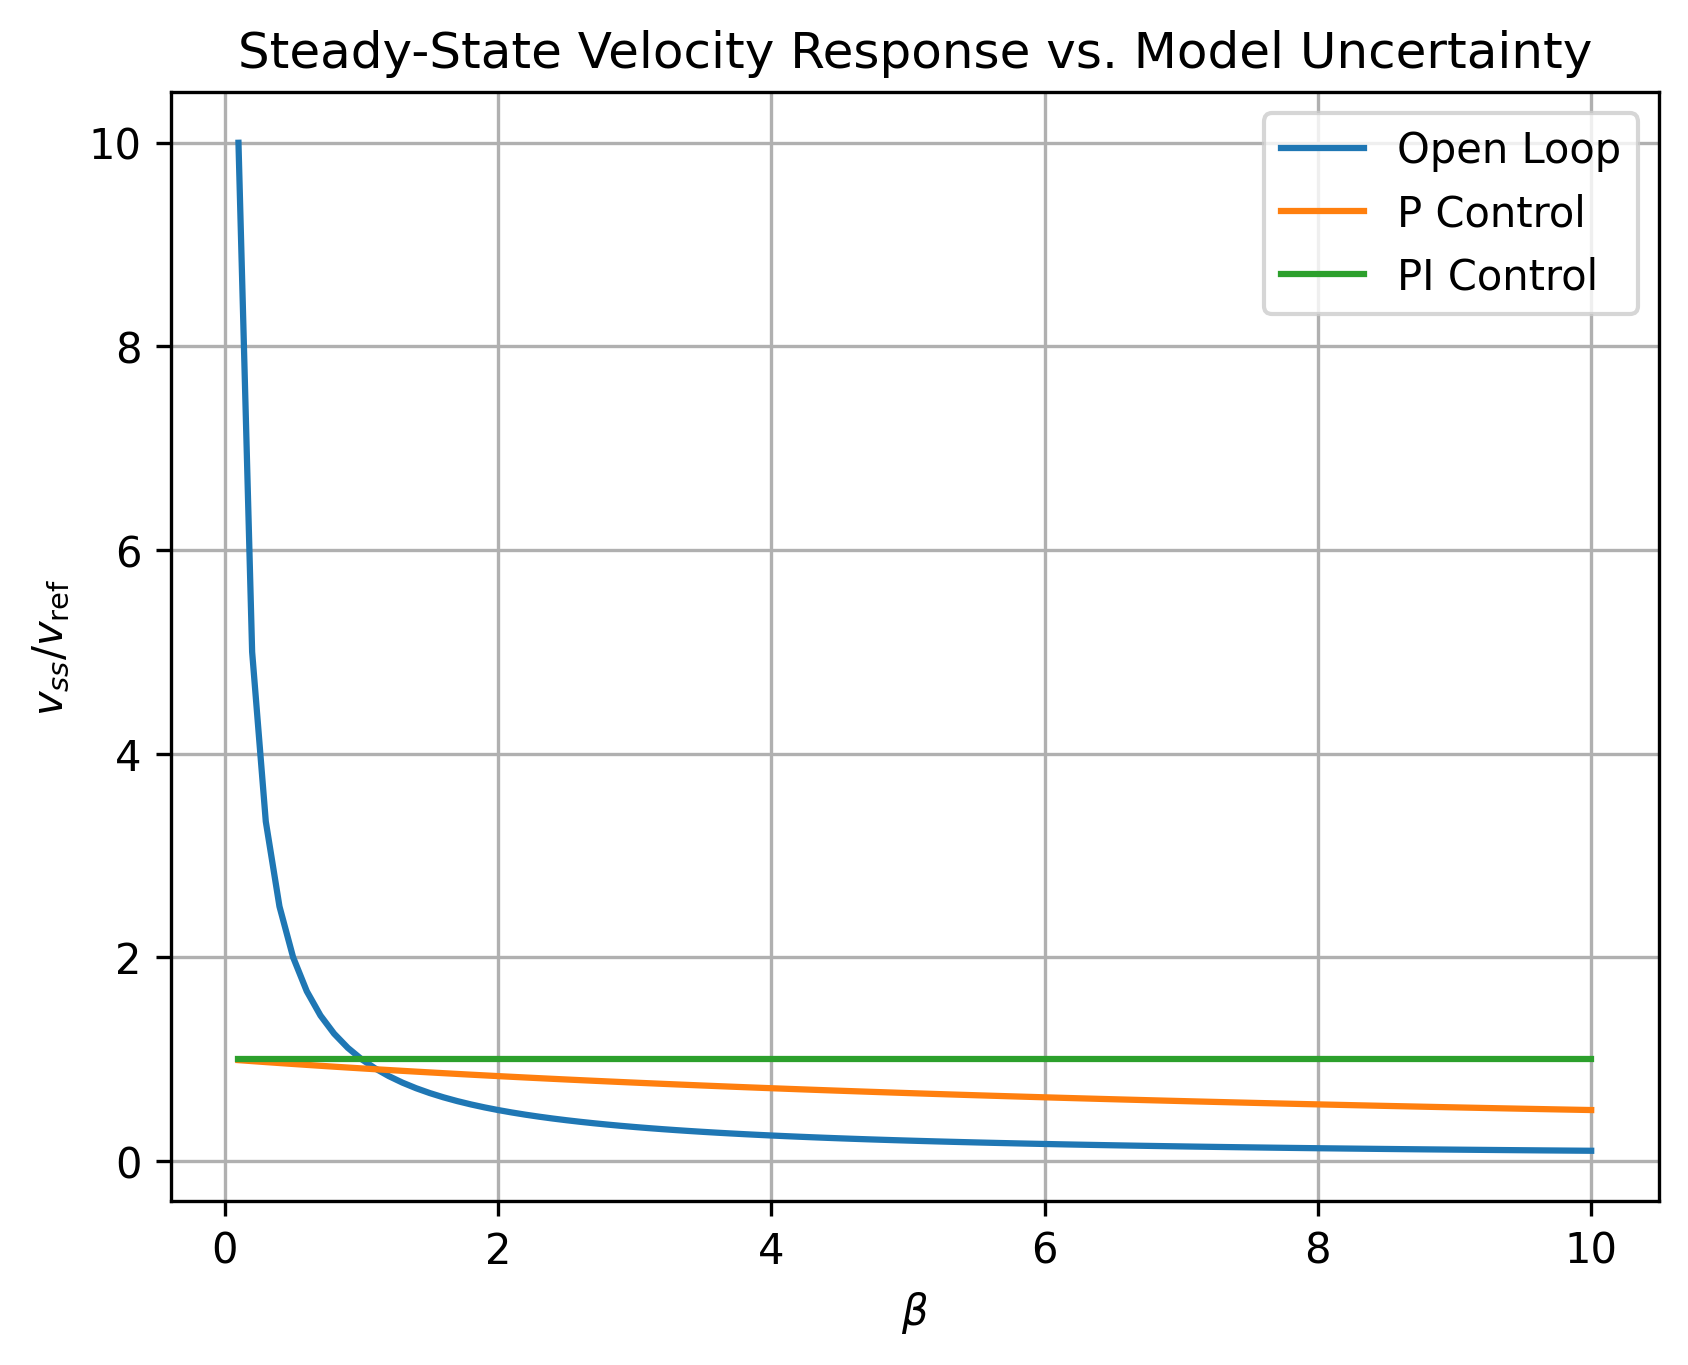
\includegraphics[width=0.7\textwidth]{HW1_4c.png}
\end{center}
\begin{enumerate}
    \item[(d)] Based on your results, briefly explain what this example demonstrates about the roles of feedforward, proportional feedback, and integral action in the presence of model uncertainty.
\end{enumerate}
\paragraph{Solution} This example shows that implementing closed loop feedback control in the form of proportional and integral control can decrease the sensitivity of a system to model uncertainty. In comparison, the open-loop feedforward control is highly sensitive to model uncertainty, as shown by the vertical asymptote in the plot above for $\beta < 1$, while the proportional feedback control does not exhibit the same asymptotic behavior and stays closer to the desired reference value (shown by how it stays closer to $v_{ss}/v_{\mathrm{ref}} = 1$). Integral control eliminates steady-state error entirely, assuming stability at equilibrium.

\subsection*{Exercise 5}
Consider the coupled spring-mass-damper system below.
\begin{center}
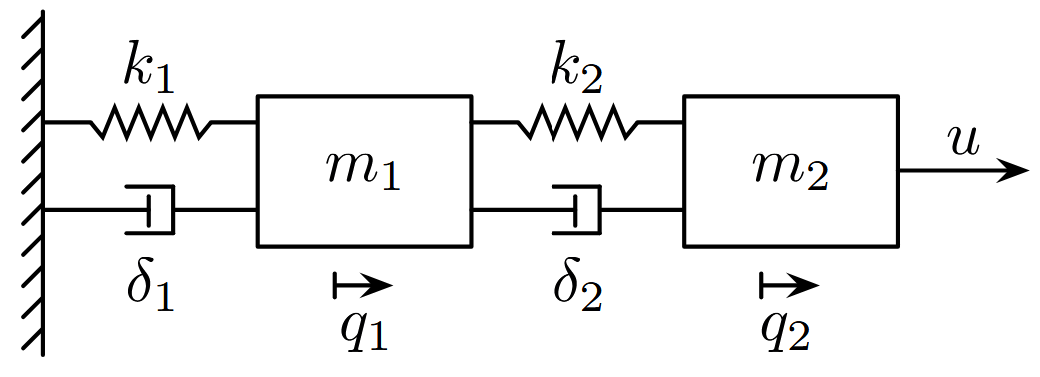
\includegraphics[width=0.5\textwidth]{Ex5.png}
\end{center}
This system is governed by the following system of coupled, second-order
ordinary differential equations:
\[
m_1\ddot{q}_1=-k_1q_1+k_2(q_2-q_1)-\delta_1\dot{q}_1+\delta_2(\dot{q}_2-\dot{q}_1),
\]
\[
m_2\ddot{q}_2=-k_2(q_2-q_1)-\delta_2(\dot{q}_2-\dot{q}_1)+u,
\]
where $q_1$ and $q_2$ are the positions of the two masses, $m_1$ and $m_2$, with respect to the lab frame. $k_1$ and $k_2$ are the spring constants, $\delta_1$ and $\delta_2$ are the damping coefficients, and $u$ is the force applied to the second mass.\\\\
Recall that state-space equations have the form
\[
\dot{\mathbf{x}}=A\mathbf{x}+B\mathbf{u},
\qquad
\mathbf{y}=C\mathbf{x}+D\mathbf{u}.
\]
Let $\mathbf{u}=u$ and $\mathbf{y}=\begin{bmatrix}q_1 & q_2\end{bmatrix}^{T}$.

\begin{enumerate}
    \item[(a)] Write the coupled ODE system above in state-space form for the state vector
    \[
    \mathbf{x}=
    \begin{bmatrix}
    x_1\\x_2\\x_3\\x_4
    \end{bmatrix}
    =
    \begin{bmatrix}
    q_1\\q_2\\\dot{q}_1\\\dot{q}_2
    \end{bmatrix}.
    \]
\end{enumerate}
\paragraph{Solution}
From the state vector definition, we have two equations:
\begin{eqnarray*}
    \dot{x_1} &=& \dot{q}_1 = x_3\\
    \dot{x_2} &=& \dot{q}_2 = x_4
\end{eqnarray*}
Rearranging the equations of motion gives the remaining two equatuions:
\begin{eqnarray*}
    \dot{x_3} &=& \ddot{q}_1 = -\left(\frac{k_1+k_2}{m_1}\right)q_1
    +\left(\frac{k_2}{m_1}\right)q_2
    -\left(\frac{\delta_1+\delta_2}{m_1}\right)\dot{q}_1
    +\left(\frac{\delta_2}{m_1}\right)\dot{q}_2\\
    \dot{x_4} &=& \ddot{q}_2 = \left(\frac{k_2}{m_2}\right)q_1
    -\left(\frac{k_2}{m_2}\right)q_2
    +\left(\frac{\delta_2}{m_2}\right)\dot{q}_1
    -\left(\frac{\delta_2}{m_2}\right)\dot{q}_2
    +\left(\frac{1}{m_2}\right)u
\end{eqnarray*}
In state-space form, we have:
\[
\dot{\mathbf{x}}
=
\begin{bmatrix}
\dot{q_1}\\\dot{q}_2\\\ddot{q}_1\\\ddot{q}_2
\end{bmatrix}
=
\begin{bmatrix}
0 & 0 & 1 & 0 \\
0 & 0 & 0 & 1 \\
-\dfrac{k_1+k_2}{m_1} & \dfrac{k_2}{m_1}
& -\dfrac{\delta_1+\delta_2}{m_1} & \dfrac{\delta_2}{m_1} \\
\dfrac{k_2}{m_2} & -\dfrac{k_2}{m_2}
& \dfrac{\delta_2}{m_2} & -\dfrac{\delta_2}{m_2}
\end{bmatrix}
\begin{bmatrix}
q_1\\q_2\\\dot{q}_1\\\dot{q}_2
\end{bmatrix}
+
\begin{bmatrix}
0 \\
0 \\
0 \\
\dfrac{1}{m_2}
\end{bmatrix}
u
\]
\[
\mathbf{y}=
\begin{bmatrix}
q_1\\q_2
\end{bmatrix}
=
\begin{bmatrix}
1 & 0 & 0 & 0 \\
0 & 1 & 0 & 0
\end{bmatrix}
\begin{bmatrix}
q_1\\q_2\\\dot{q}_1\\\dot{q}_2
\end{bmatrix}
+
\begin{bmatrix}
0 \\
0
\end{bmatrix}
u
\]
\begin{enumerate}
    \item[(b)] Write the coupled ODE system above in state-space form for the state vector
    \[
    \tilde{\mathbf{x}}=
    \begin{bmatrix}
    \tilde{x}_1\\\tilde{x}_2\\\tilde{x}_3\\\tilde{x}_4
    \end{bmatrix}
    =
    \begin{bmatrix}
    q_1\\q_2-q_1\\\dot{q}_1\\\dot{q}_2-\dot{q}_1
    \end{bmatrix}.
    \]
\end{enumerate}
\paragraph{Solution} From the state vector definition, we have two equations:
\begin{eqnarray*}
    \dot{\tilde{x}}_1 &=& \dot{q}_1 = \tilde{x}_3\\
    \dot{\tilde{x}}_2 &=& \dot{q}_2-\dot{q}_1 = \tilde{x}_4
\end{eqnarray*}
Rearranging the equations of motion gives the remaining two equatuions:
\begin{eqnarray*}
    \dot{\tilde{x}}_3 &=& \ddot{q}_1 = \frac{-k_1}{m_1} q_1
    -\frac{k_2}{m_1}(q_2-q_1)
    -\frac{\delta_1}{m_1}\dot{q}_1
    -\frac{\delta_2}{m_1}(\dot{q}_2-\dot{q}_1)\\
    \implies \dot{\tilde{x}}_3 &=& \frac{-k_1}{m_1} \tilde{x}_1
    -\frac{k_2}{m_1}\tilde{x}_2
    -\frac{\delta_1}{m_1}\tilde{x}_3
    -\frac{\delta_2}{m_1}\tilde{x}_4\\
    \dot{\tilde{x}}_4 + \ddot{q}_1 &=& \ddot{q}_2 = \frac{k_2}{m_2}(q_2-q_1)
    -\frac{\delta_2}{m_2}(\dot{q}_2-\dot{q}_1)
    +\frac{1}{m_2}u\\
    \implies \dot{\tilde{x}}_4 &=& \frac{k_2}{m_2} \tilde{x}_2 - \frac{\delta_2}{m_2}\tilde{x}_4 + \frac{1}{m_2}u - \dot{\tilde{x}}_3\\
    \implies \dot{\tilde{x}}_4 &=& \frac{k_2}{m_2} \tilde{x}_2 - \frac{\delta_2}{m_2}\tilde{x}_4 + \frac{1}{m_2}u - \left[\frac{-k_1}{m_1} \tilde{x}_1
    -\frac{k_2}{m_1}\tilde{x}_2
    -\frac{\delta_1}{m_1}\tilde{x}_3
    -\frac{\delta_2}{m_1}\tilde{x}_4\right]\quad \text{(substitute in for } \dot{\tilde{x}}_3 )\\
    \implies \dot{\tilde{x}}_4 &=& \frac{k_1}{m_1} \tilde{x}_1
    +\left(\frac{k_2}{m_2}+\frac{k_2}{m_1}\right)\tilde{x}_2
    +\frac{\delta_1}{m_1}\tilde{x}_3
    +\left(\frac{\delta_2}{m_1}-\frac{\delta_2}{m_2}\right)\tilde{x}_4
    +\frac{1}{m_2}u
\end{eqnarray*}
The state-space form is then:
\[
\dot{\tilde{\mathbf{x}}}
=
\begin{bmatrix}
\dot{q}_1\\
\dot{q}_2-\dot{q}_1\\
\ddot{q}_1\\
\ddot{q}_2-\ddot{q}_1
\end{bmatrix}
=
\begin{bmatrix}
0 & 0 & 1 & 0\\
0 & 0 & 0 & 1\\
-\dfrac{k_1}{m_1}
&
-\dfrac{k_2}{m_1}
&
-\dfrac{\delta_1}{m_1}
&
-\dfrac{\delta_2}{m_1}
\\
\dfrac{k_1}{m_1}
&
\dfrac{k_2}{m_1}+\dfrac{k_2}{m_2}
&
\dfrac{\delta_1}{m_1}
&
\dfrac{\delta_2}{m_1}-\dfrac{\delta_2}{m_2}
\end{bmatrix}
\begin{bmatrix}
q_1\\
q_2-q_1\\
\dot{q}_1\\
\dot{q}_2-\dot{q}_1
\end{bmatrix}
+
\begin{bmatrix}
0\\
0\\
0\\
\dfrac{1}{m_2}
\end{bmatrix}
u
\]
For the output matrix, we have:
\begin{eqnarray*}
    q_1 &=& \tilde{x}_1\\
    q_2 &=& \tilde{x}_1 + \tilde{x}_2
\end{eqnarray*}
\[
\mathbf{y}
=
\begin{bmatrix}
q_1\\
q_2
\end{bmatrix}
=
\begin{bmatrix}
1 & 0 & 0 & 0\\
1 & 1 & 0 & 0
\end{bmatrix}
\begin{bmatrix}
q_1\\
q_2-q_1\\
\dot{q}_1\\
\dot{q}_2-\dot{q}_1
\end{bmatrix}
+
\begin{bmatrix}
0\\
0
\end{bmatrix}
u
\]
\begin{enumerate}
    \item[(c)] Write the second state vector in terms of the first. What does this relationship tell you about the two state-space models? Hint: Can you find a matrix $T$ such that $\tilde{\mathbf{x}}=T\mathbf{x}$?
\end{enumerate}
\paragraph{Solution} Following the hint:
\[\tilde{\mathbf{x}} = 
\begin{bmatrix}
1 & 0 & 0 & 0\\
-1 & 1 & 0 & 0\\
0 & 0 & 1 & 0\\
0 & 0 & -1 & 1
\end{bmatrix}
\begin{bmatrix}
q_1\\q_2\\\dot{q}_1\\\dot{q}_2
\end{bmatrix} =
\begin{bmatrix}
q_1\\
q_2-q_1\\
\dot{q}_1\\
\dot{q}_2-\dot{q}_1
\end{bmatrix}\]
This relationship shows that second state vector is a linear transformation of the first state vector while describing the same system dynamics. Physically, the second state vector describes the position and velocity of the second mass relative to the first mass instead of relative to the lab frame.
\end{document}
